\newcommand{\PaperSummary}{We analyze 108 calls and 139 paired playback experiments in four linked models. A grouped acoustic classifier using six shared measurements gives macro F1 of 0.225, compared with 0.207 for the fold-majority model. At a fidelity threshold of 0.50, flat, modulated and two-voice calls have acoustic ranges of 84.7, 144.6 and 169.7 m. Natural calls elicited a response in 90 of 139 playbacks, compared with 18 of 139 controls. The observed paired difference was 51.8 percentage points, with a 95\% paired bootstrap interval of 43.9--60.1 points. The integrated clean effectiveness radii are 87.0 m, 131.7 m and at least 150 m, respectively. Under a modeled 20\% fidelity loss, those distances fall to 46.0, 70.4 and 124.3 m. We report the uncertainty and sensitivity of these operational distances and outline a field design for evaluating noise in foraging areas.}

\newcommand{\AcousticResults}{Peak frequency was the only acoustic measure reaching 5\% in the Holm-adjusted omnibus tests ($p=0.0130$). The significant pairwise difference was flat versus modulated peak frequency ($p=0.0244$). The grouped macro F1 was 0.225 with a recording-group bootstrap range of 0.145--0.286, versus 0.207 for the majority baseline. Adding median-imputed pulse rate gave 0.259. Pulse rate was absent in all flat calls and missing in some modulated and two-voice calls. Availability of F02 alone gave 0.569 because F02 was recorded only for the two-voice category. Held-out permutation scores did not identify a stable positive contribution from a shared feature. We carry the supplied call labels into propagation and behavior modeling. The peak-frequency result motivates retaining a spectral component in the fidelity measure. The weak grouped classifier supports using measured call labels rather than assigning new labels from acoustic features.
\par\begin{center}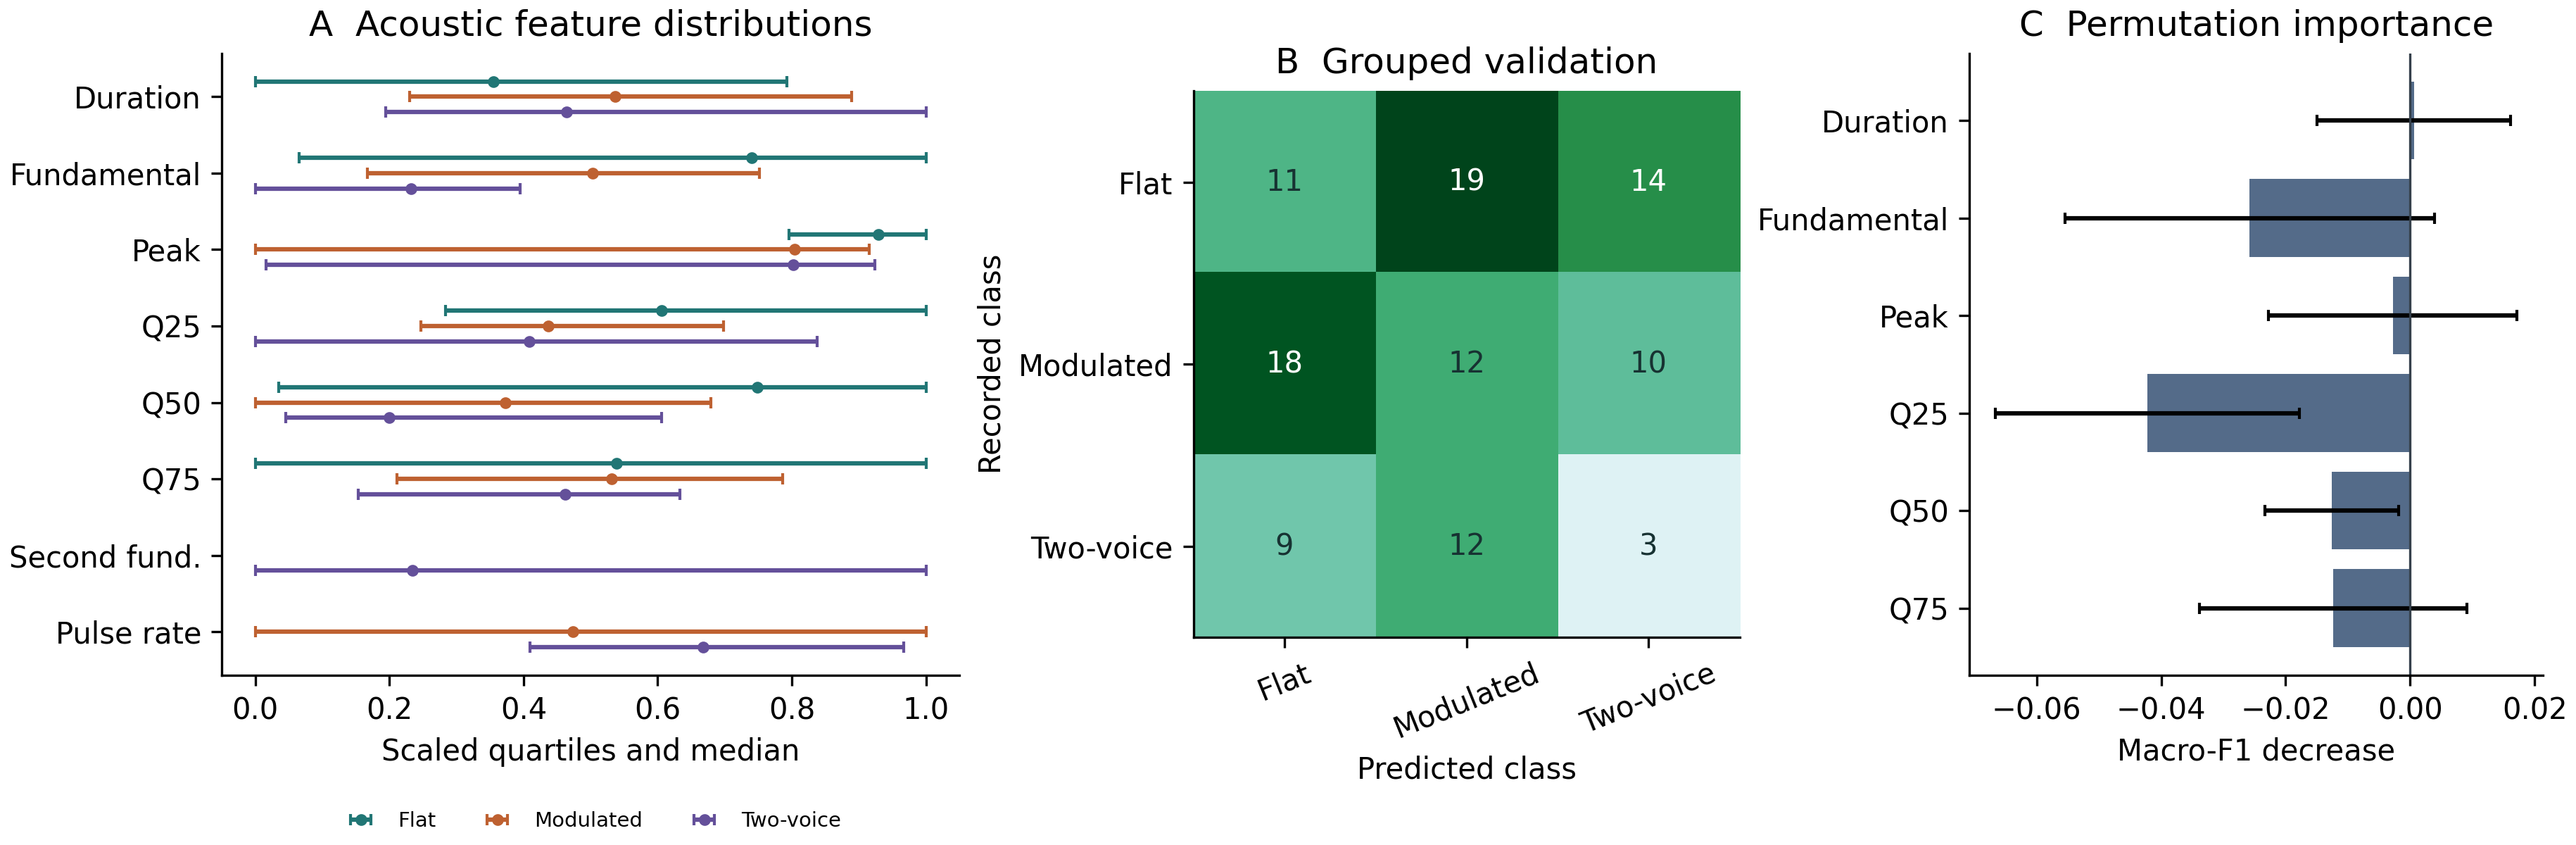
\includegraphics[width=.92\linewidth]{q1_acoustics.png}\\
{\small Figure 1. Acoustic summaries, grouped classification and held-out permutation importance.}\end{center}}

\newcommand{\PropagationResults}{
\begin{center}\small
\begin{tabular}{lrrr}
\toprule
Call & 0.40 & 0.50 & 0.60\\
\midrule
Flat & 113.5 [111.8,115.2] & 84.7 [83.7,85.9] & 62.6 [60.6,64.4]\\
Modulated & 181.7 [180.0,183.9] & 144.6 [142.3,147.1] & 109.2 [106.9,112.0]\\
Two-voice & 203.9 [202.7,205.1] & 169.7 [168.9,170.6] & 141.3 [140.5,142.0]\\
\bottomrule
\end{tabular}\\[3pt]
Table 1. Propagation ranges in metres, with 95\% conditional bootstrap intervals.
\end{center}
Two-voice has the longest estimated range at the three primary thresholds under the tested weights. At 0.70, the equal-weight estimate for two-voice is close to that for modulated calls and their uncertainty intervals overlap. Increasing the envelope weight can reverse their ranking at 0.70. Choice of the similarity criterion therefore matters most for claims about very reliable recognition.
\par\begin{center}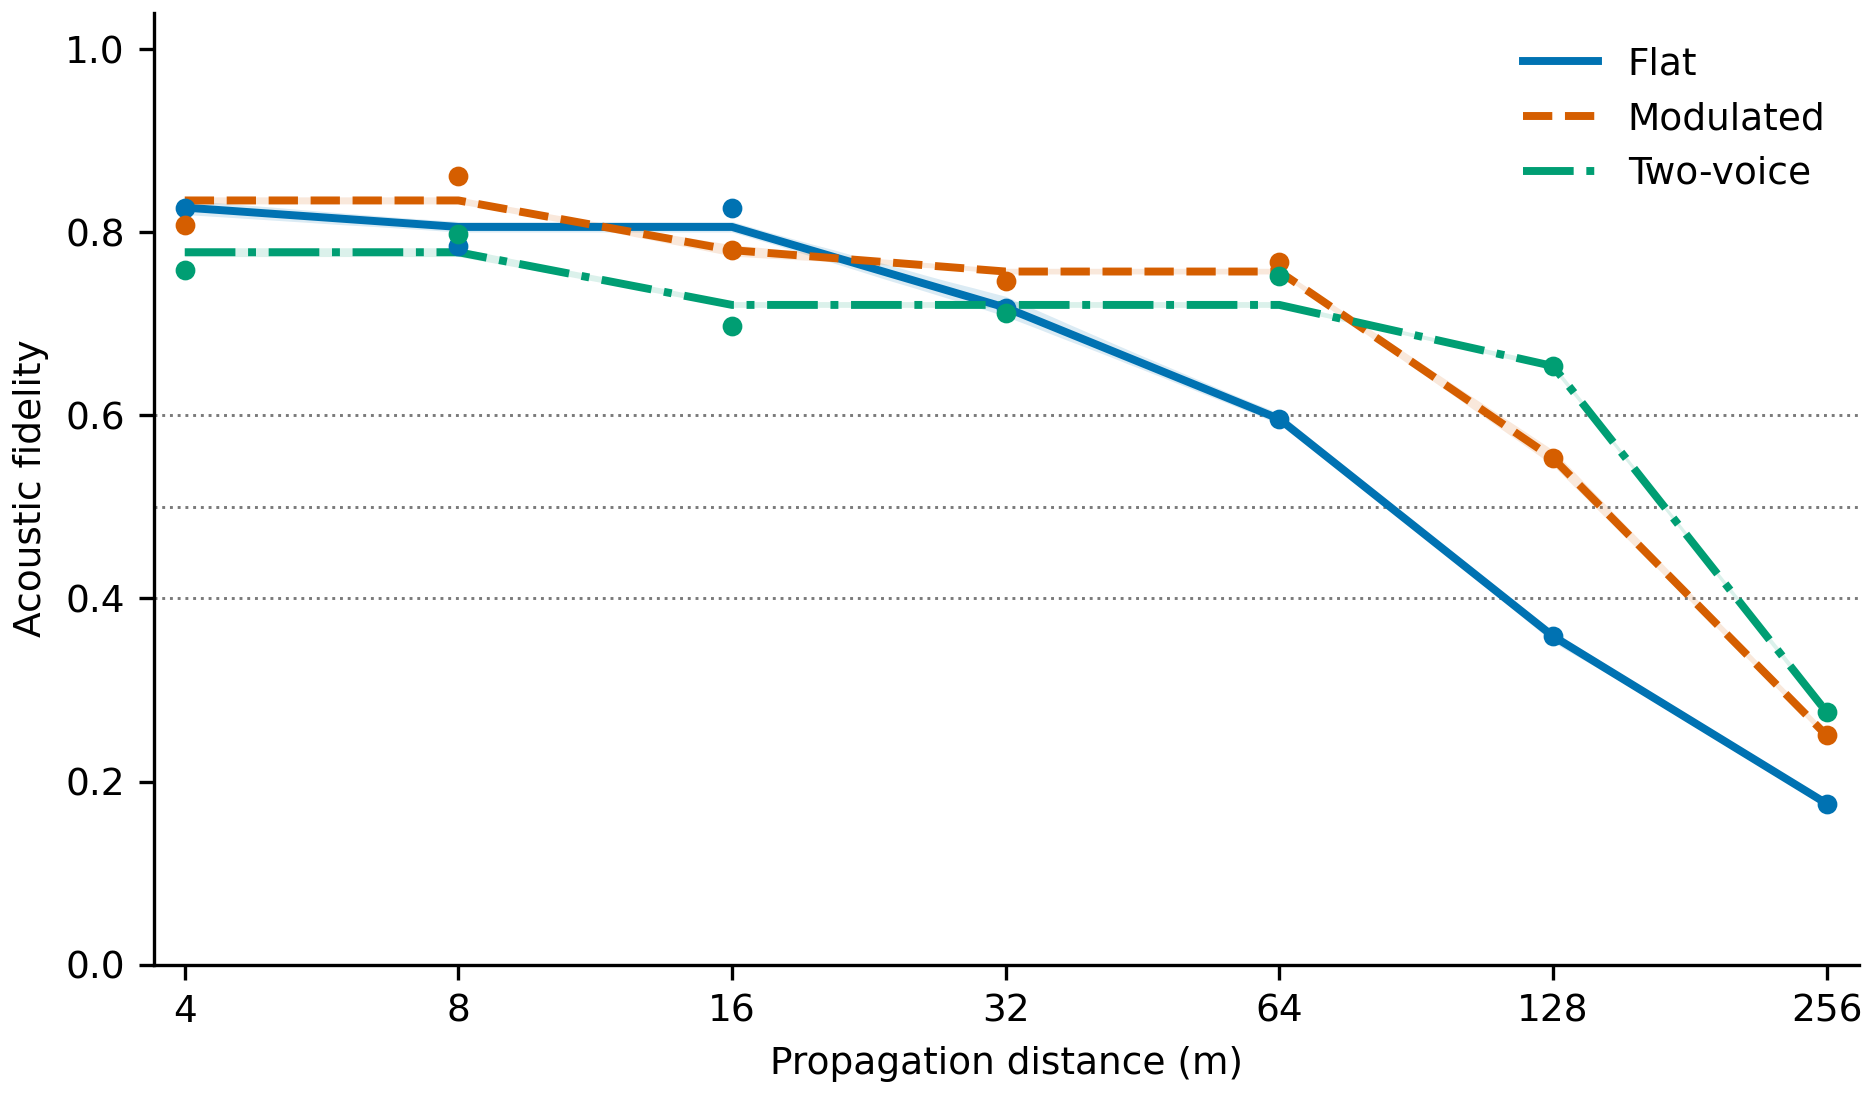
\includegraphics[width=.94\linewidth]{q2_propagation.png}\\{\small Figure 2. Equal-weight fidelity and conditional propagation intervals.}\end{center}}

\newcommand{\BehaviorResults}{
There were 74 pairs with a response only to the natural call, two with a response only to control, 16 with both and 47 with neither. The exact McNemar $p$ value was $7.75\times10^{-20}$ for equality of the observed paired marginal response rates. With grouped validation, the multinomial model had a mean mask log loss of 1.245, versus 1.384 for pooled training frequencies. The corresponding Brier scores for any response were 0.154 and 0.238. At 50 m and eight observed birds, the adjusted natural-call increment for the vocal-only response to flat calls was 0.134, with an interval of 0.043--0.276. The full combination distribution includes joint responses and baseline controls.
\par\begin{center}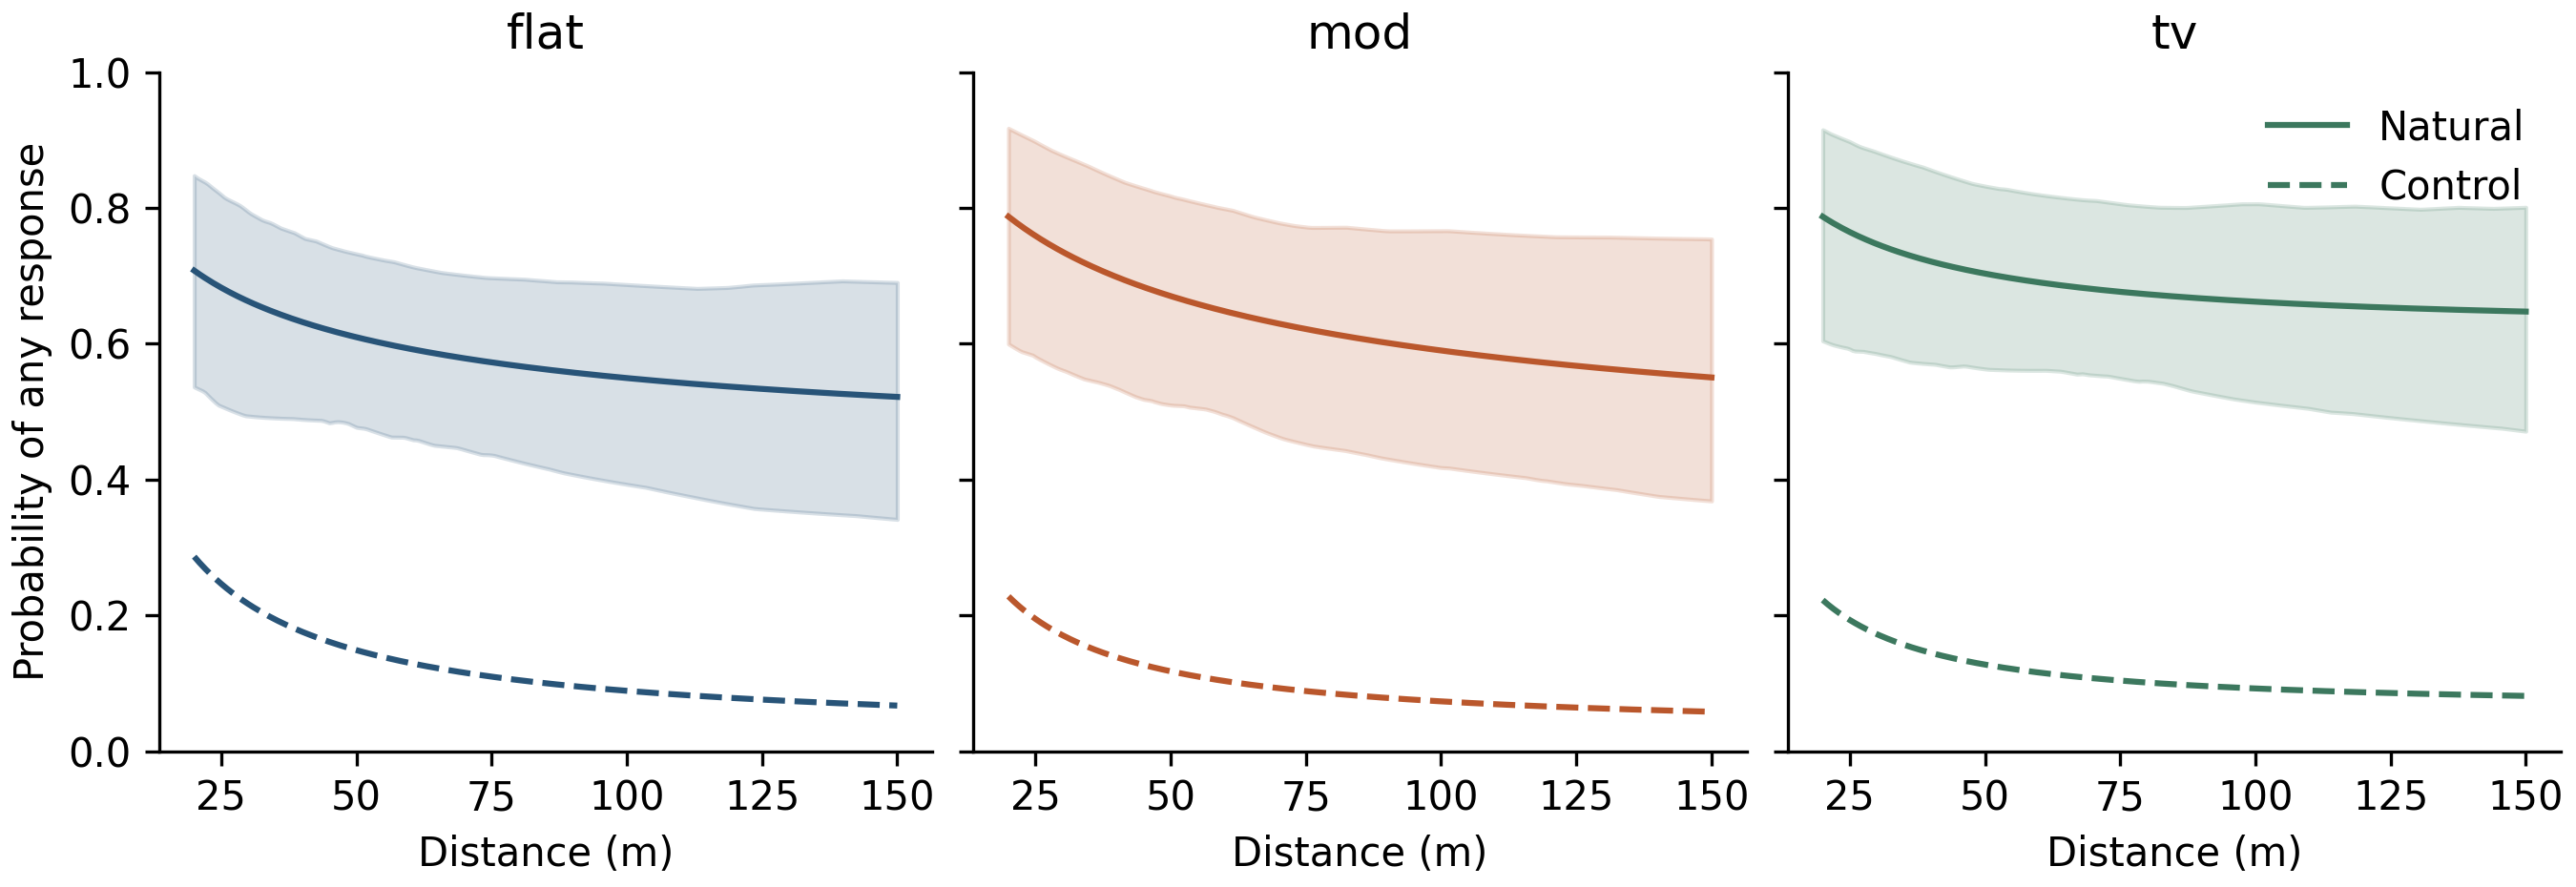
\includegraphics[width=.87\linewidth]{q3_response_curve.png}\\{\small Figure 3. Adjusted any-response probabilities. Shading shows paired bootstrap intervals for natural stimuli.}\end{center}
\begin{center}\small
\begin{tabular}{lrrr}
\toprule
Call & 50 m & 100 m & 150 m\\
\midrule
Flat & 1.79 & 1.88 & 1.94\\
Modulated & 1.81 & 1.91 & 1.96\\
Two-voice & 2.10 & \TVHundred & \TVFar\\
\bottomrule
\end{tabular}\\[3pt]
Table 2. Predicted median onset of head raising in seconds, conditional on head raising, for natural calls and eight birds.
\end{center}
At 150 m, the flat and modulated onset estimates use information pooled from the wider dataset because no observed head-raising onsets occur within 25 m in those call strata. Control stimuli produced no observed approaches, leaving their conditional approach onset unavailable. Tables accompanying the paper contain each behavior's probabilities and latency estimates at all three distances, along with the vocal-count and duration summaries.}

\newcommand{\IntegratedResults}{
\begin{center}\small
\begin{tabular}{lrrr}
\toprule
Call & Clean & 20\% loss & Threshold 0.70\\
\midrule
Flat & 87.0 & 46.0 & 35.2\\
Modulated & 131.7 & 70.4 & 77.6\\
Two-voice & $\ge 150$ & 124.3 & 79.2\\
\bottomrule
\end{tabular}\\[3pt]
Table 3. Integrated radii in metres, using the fixed 50\% clean reference.
\end{center}
The clean flat radius has a conditional bootstrap range of 64.8--121.0 m. The modulated and two-voice intervals reach the upper study bound. At the same relative criterion, the behavior-only model reaches the support limit for every call. Integrating the acoustic component provides an in-range crossing for flat and modulated calls. The acoustic-only radius for flat calls is 117.3 m and the integrated estimate is 87.0 m. At 100 m, the modeled 20\% loss changes response probabilities from 0.549, 0.590 and 0.662 to 0.457, 0.487 and 0.548 for flat, modulated and two-voice calls, respectively. If half of an eight-bird responding group participates, those three altered probabilities imply mean counts of about 1.83, 1.95 and 2.19. The rank in the clean point estimates is stable across the two alternative acoustic weights, with the two-voice result bounded by support.
\par\begin{center}\begin{minipage}{.94\linewidth}\centering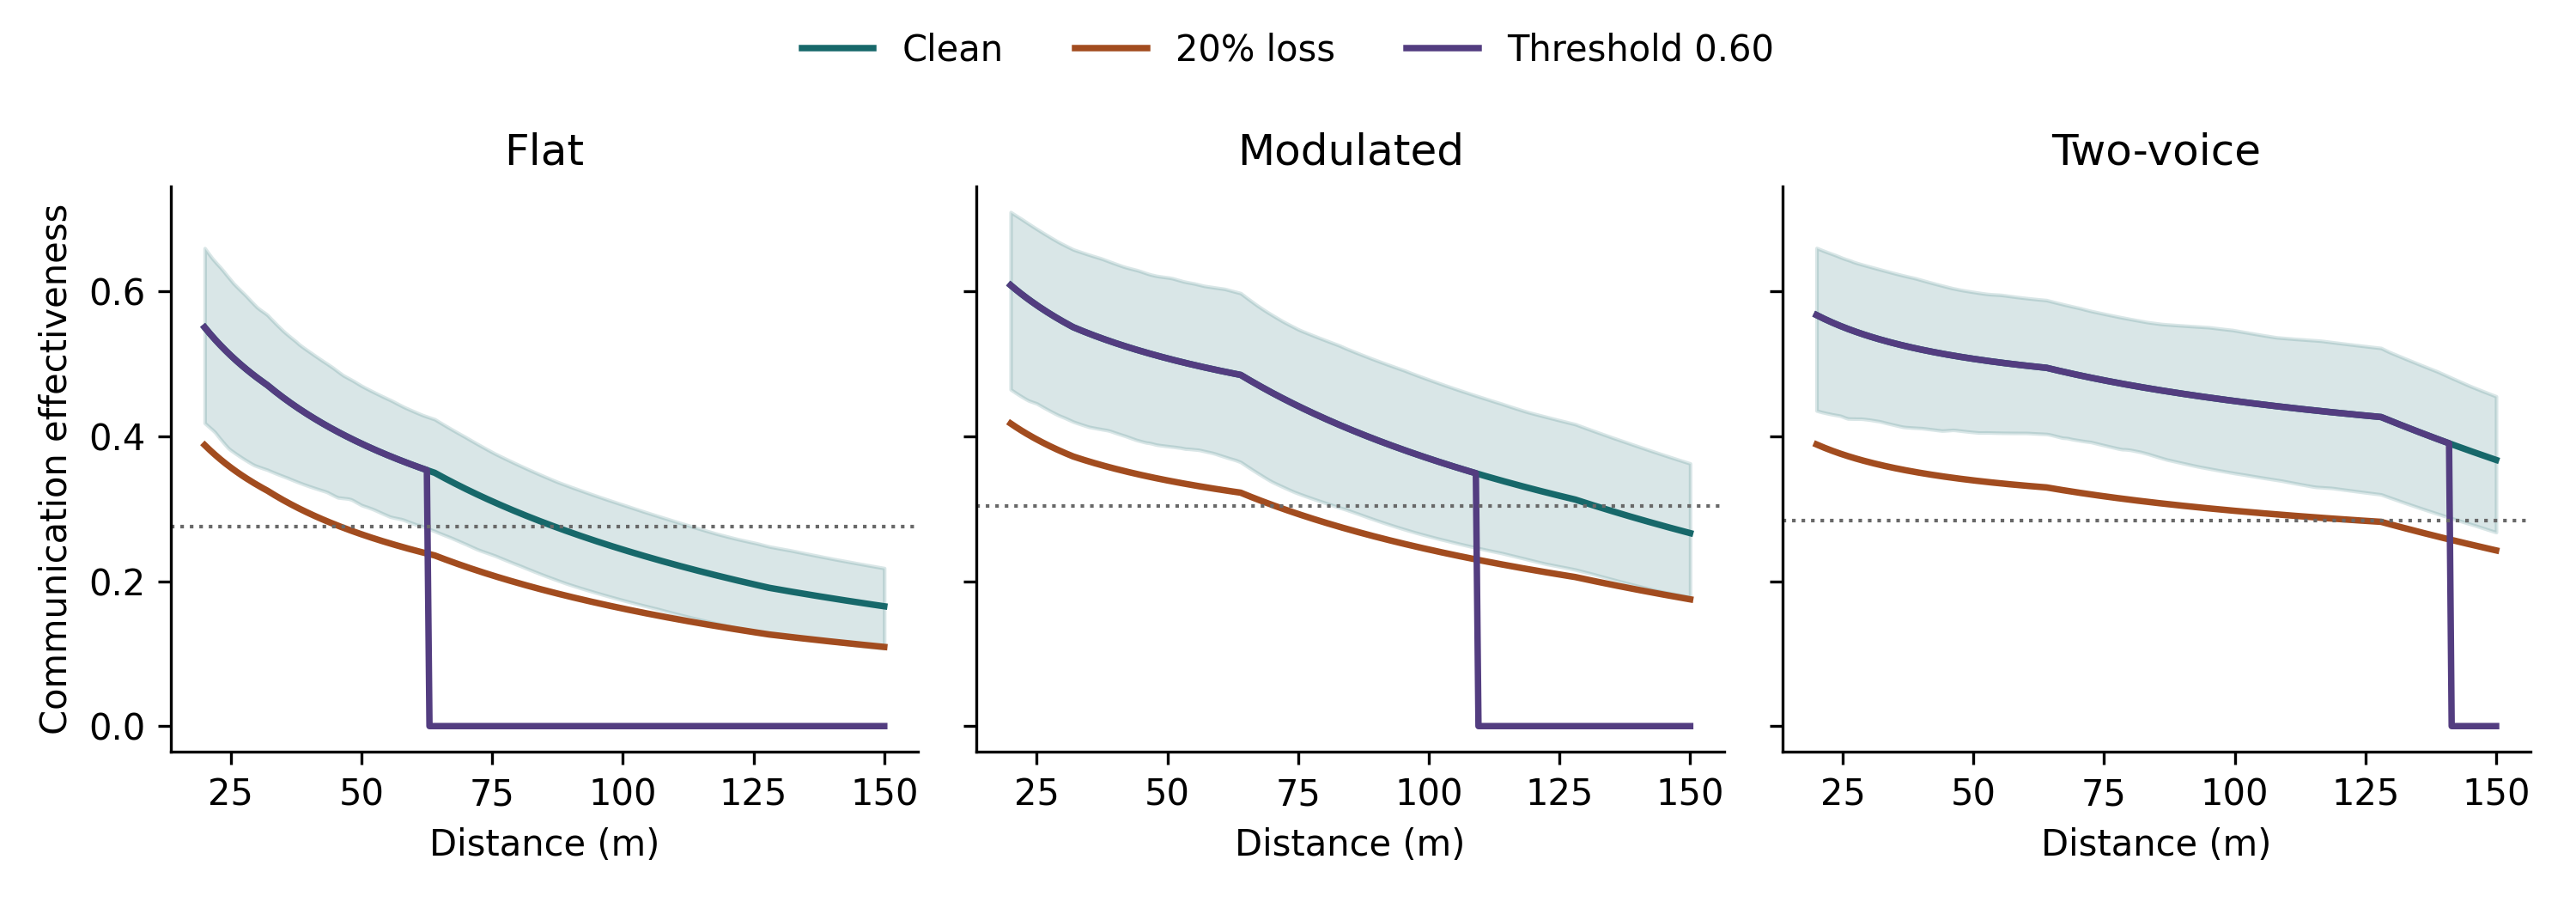
\includegraphics[width=\linewidth]{q4_scenarios.png}\\{\small Figure 4. Integrated effectiveness by distance. Dotted lines mark the fixed clean reference and shading shows the clean conditional interval.}\end{minipage}\end{center}}

\newcommand{\TVHundred}{2.20}
\newcommand{\TVFar}{2.26}



